\chapter{Theoretical analysis of the~KSA}

This thesis is /red{focused on deriving/ on derivation of} the secret key from the inner state after the KSA. This is possible thanks to the fact, that the permutation after the KSA algorithm is biased towards the secret key. From the aforementioned attacks we focus on a class of key retrieval algorithms which uses this fact to extract complete key or information about some of its bytes. 

There are different types in biases in the permutation after the KSA. Later we will use some of them in the key retrieval algorithm to extract the secret key with certain probability. 



It was first experimentally observed by Roos in 1995 \cite{roos} that the most likely value of the inner permutation, denoted $ S_{N}$, is given by 
\[ S_{N}[i] = \dfrac{i(i+1)}{2} + \K{0}{i} \]
 This equation holds with high probability for roughly 40 initial entries. Theoretical analysis was later provided by G. Paul and S. Maitra in \red{\cite{GoMa}} and subsequently generalized by \red{citace} as follows:
 \[ S_{N}[i_{2}] - S_{N}[i_{1}] = \K{i_{1}+1}{i_{2}} + \dfrac{i_{2}(i_{2}+1)}{2} - \dfrac{i_{1}(i_{1}+1)}{2} \]
Which has high probability also with higher indices and can be used together with tools described bellow to effectively retrieve the secret key. 



%%%%%%%%%%% Notations                %%%%%%%%%%%%
%%%%%%%%%%%%%%%%%%%%%%%%%%%%%%%%%%%%%%%%%%%%%%%%%
\section{Notations and basic assumptions}

\begin{notation}
	
	Let $ K $ be an array of key bytes of length $ l $. $ K[a] $ will always be understood as $ K[a \Mod{l}] $ and we will write
	
	\[\K{a}{b} \coloneqq \sum\limits_{i=a}^{b}K[i \Mod{l}]. 	\]
	
	 
	
	The index $ j $ in $ r $-th round of the KSA will be denoted by $ j_{r} $,  $ S_{r} $ denotes the permutation after $ r $-th round of the KSA.  Therefore $ S_{N} $ is the permutation after complete KSA. For simplicity, $ S $ without index will mean $ S_{N} $, i.e. the permutation after the complete KSA. 	
	$ 	\InvS $ will stand for the inverse permutation of $ S $, i.e. $ \forall y \in \FromTo{0}{N-1}: S[y] = v \Rightarrow \InvS[v] = y$. 
	

	
\end{notation}


%%%%%%%%%%% Prvni bias %%%%%%%%%%%%%%%%%%%%%%%%%%
%%%%%%%%%%%%%%%%%%%%%%%%%%%%%%%%%%%%%%%%%%%%%%%%%

\section{Bias towards the sequence sums of key bytes}

	In the KSA, in every round the index $ i $ is incremented by one and the pseudorandom index $ j $ is calculated by following rule:
	\[  j_{i+1} = j_{i} + S_{i}[i] + K[i] \]


	 
	If we recursively substitute for $ j $, we can write the update rule in the following form:
	\[ 
	j_{i+1} = \sum_{r=0}^{i}S_{r}[r] + \sum_{r=0}^{i}K[r]
	.\]
	
	Assuming that $ S_{i}[i] = i $ we obtain 
	\[
	 j_{i+1} = \sum_{r=0}^{i}r + \sum_{r=0}^{i}K[r] = \dfrac{i(i+1)}{2} + \K{0}{i}
	.\]
	
	\TODO{ODSTRANIT Y ----> I}
	 
	 We will show, that with certain probability $ S_{N}[i] = S_{r}[i] = j_{i+1}$, therefore 
 	\[ S_{N}[i] = \dfrac{i(i+1)}{2} + \K{0}{i} \].
 	
 	
 	Despite $ j $ being updated using deterministic formula, it is a linear function of a pseudorandom key and therefore itself pseudorandom. Thanks to that we can consider $ j $ as being random.
 	
 	
	 	

	%%%%%%%%%%% Lemma 1                %%%%%%%%%%%%
	\begin{lemma}
		Assume that the index $ j $ takes its value from $ \Z_{N}  $ uniformly at random at each round of the KSA. Then $ \forall i \in \Z_{N} $:
		\begin{equation}\label{lemma1}
		\Pr \left(j_{i+1} = \dfrac{i(i+1)}{2} + \K{0}{i}\right) \approx \left(\dfrac{N-1}{N}\right)^{1+\frac{i(i+1)}{2}} + \dfrac{1}{N} 
		\end{equation}	

	\end{lemma}		


	\begin{proof}
		Let $ E_{i} $ denote the event that 
		\[ j_{i+1} = \sum_{r=0}^{i}(i + K[r])\]
		
		and $ A_{i} $ denote the event that
		\[\forall r \in [0,i]: \ S_{r}[r] = r   \].
		
		From the law of total probability \ref{totalProb} we have
		
		\[ \Pr(E_{i}) = 
		\Pr(E_{i} \cond A_{i})\Pr(A_{i}) 
		+   \Pr(E_{i} \cond \complem{A_{i}})\Pr(\complem{A_{i}}) \] 
			
			
		Index $ j $ is uniformly distributed, hence $ \Pr(E_{i}|\complem{A_{i}}) \approx \dfrac{1}{N} $ and from the reasoning above, $ \Pr(E_{i} \cond A_{i}) = 1 $. 	
		
		We will show by induction that
		
		\[ \Pr(A_{i}) = \bigg(\dfrac{N-1}{N}\bigg)^{\frac{i(i+1)}{2}}.\]
		
		The case $ \Pr(A_{0} = 1) $ is trivial. For $ i \geq 1 $
		
		\begin{align*}
			\Pr(A_{i})  &= \Pr(A_{i-1} \, \cap \, (S_{i}[i] = i) )
					 \\ &= \Pr(A_{i-1})\cdot\Pr((S_{i}[i] = i) ) \text{ \red{nezavisle, zminit?}}
					 \\ &\stackrel{IH}{=} \bigg(\dfrac{N-1}{N}\bigg)^{\frac{(i-1)i}{2}}\cdot\Pr((S_{i}[i] = i) ) 
					 \\ &= 
					 \bigg(\dfrac{N-1}{N}\bigg)^{\frac{(i-1)i}{2}}
					 \bigg(\dfrac{N-1}{N}\bigg)^{i}
					 \\ &= 
					 \bigg(\dfrac{N-1}{N}\bigg)^{\frac{i(i+1)}{2}}
		\end{align*}		
		It is worth mentioning that we used the fact that the events $ A_{i} $ and $ S_{i}[i] = i $ are independent. Together we get
		
				
			\begin{align*}
				\Pr(E_{i}) &= \Pr(E_{i} \cond A_{i})\Pr(A_{i}) 
						    + \Pr(E_{i} \cond \complem{A_{i}})\Pr(\complem{A_{i}}) 
				\\ &\approx 1 \cdot \bigg(\dfrac{N-1}{N}\bigg)^{\frac{i(i+1)}{2}} 
				            + \dfrac{1}{N}\bigg(1-\bigg(\dfrac{N-1}{N}\bigg)^{\frac{i(i+1)}{2}} \bigg)
				\\ &= \bigg(\dfrac{N-1}{N}\bigg)^{\frac{i(i+1)}{2}} + \dfrac{1}{N} -
								\dfrac{1}{N}\bigg(\dfrac{N-1}{N}\bigg)^{\frac{i(i+1)}{2}}	
				\\ &= \bigg(\dfrac{N-1}{N}\bigg)^{\frac{i(i+1)}{2}} \cdot \bigg( 1 - \dfrac{1}{N}\bigg)
				+ \dfrac{1}{N}
				\\ &= \bigg(\dfrac{N-1}{N}\bigg)^{1+\frac{i(i+1)}{2}} + \dfrac{1}{N}	
			\end{align*}
			
			which completes the proof.	
		
	\end{proof}	
	

		
	
	\TODO{kdyz se shoduje s experimenty, tak nakreslit jen rovnici? A proc je tak mimo dole?}
	
	\begin{figure}
\centering
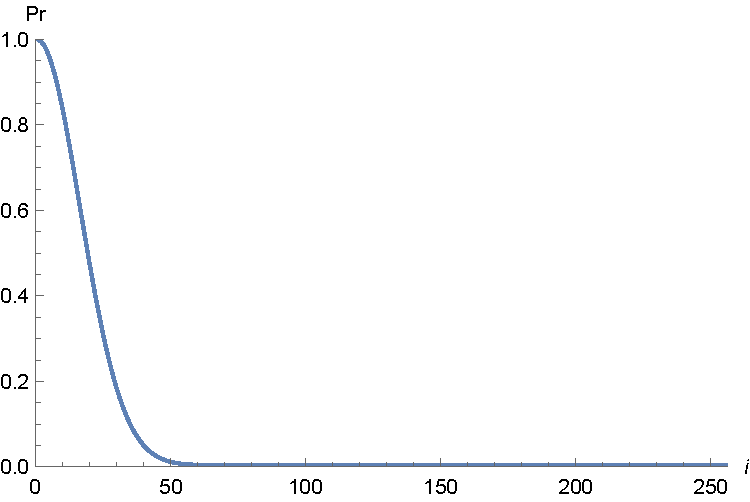
\includegraphics[width=0.7\linewidth]{img/lemma1}
\caption{$ \Pr\Big(j_{i+1} = \dfrac{i(i+1)}{2} + \K{0}{i} \Big) $}
\label{fig:lemma1}
\end{figure}




	%%%%%%%%%%% Lemma 2                %%%%%%%%%%%%%%% 	
	\begin{lemma}
	Assume that the index $ j $ takes its value from $ \Z_{N} $ independently
	and uniformly at random at each round of the KSA. Then, for the permutation after the KSA, $ 0~\leq~i~\leq~N-1 $
	\begin{equation}\label{lemma2}
	\Pr(S_{N}[i] = j_{i+1}) \approx \bigg(\dfrac{N-i}{N}\bigg)\bigg(\dfrac{N-1}{N}\bigg)^{N-1}
	\end{equation}
	\end{lemma}
	\begin{proof}
		In round $ i+1 $ elements of the permutation $ S $ on positions $ i $ and $ j_{i+1} $ are swapped. Therefore $ S_{i+1}[i] = S_{i}[j_{i+1}] $.
		
		Lemma holds under these assumptions:
		\begin{enumerate}
			\item $ j_{r} \neq j_{i} $ for $ r \in \FromTo{0}{i-1}$, i.e. $ S[j_{i}] $ is not swapped until the $ i $-th iteration.
			\item $ j_{i} \geq i $, i.e. $ S[i] $ is swapped with item with greater index.
			\item $ j_{r} \neq i $ for $ r \in \FromTo{i+1}{N-1}$, i.e. $ S[i] $ is involved in remaining rounds. 
		\end{enumerate} 
		
		$ S_{i}[j_{i+1}] = j_{i+1} $ if this element is not involved in any of the previous rounds. This \red{happens} if and only if $ j_{i+1} \notin \FromTo{0}{i-1} \cup \FromTo{j_{1}}{j_{i}} $.
		
		$ \Pr(j_{i+1} \notin \FromTo{0}{i-1}) = \left(\dfrac{N-i}{N}\right) $ and
		$ \Pr(j_{i+1} \notin \FromTo{j_{0}}{j_{i}}) = \left(\dfrac{N-1}{N}\right)^{i} $,
		hence 
		
		\[ \Pr(S_{i+1}[i] = j_{i+1}) = \bigg( \dfrac{N-i}{N}\bigg)
									\bigg( \dfrac{N-1}{N}\bigg)^{i}.\]
		If in next $ N-1-i $ rounds the index $ i $ is not touched by any of the subsequent $ j $ indices, i.e. $ \forall r \in \FromTo{i+1}{N} \; j_{r} \neq i $, the value will stay on place, thus 	$ S_{N}[j_{i+1}] = j_{i+1} $.  This holds with probability $(\frac{N-1}{N})^{N-1-i} $. Together we get
		
		\[\Pr(S_{N}[i] = j_{i+1}) =  \bigg( \dfrac{N-i}{N}\bigg)
		\bigg( \dfrac{N-1}{N}\bigg)^{i}
		\bigg( \dfrac{N-1}{N}\bigg)^{N-1-i}. \]
		
	\end{proof}


Experimental data \TODO{popisky v mathematice}

	\begin{figure}
		\centering
		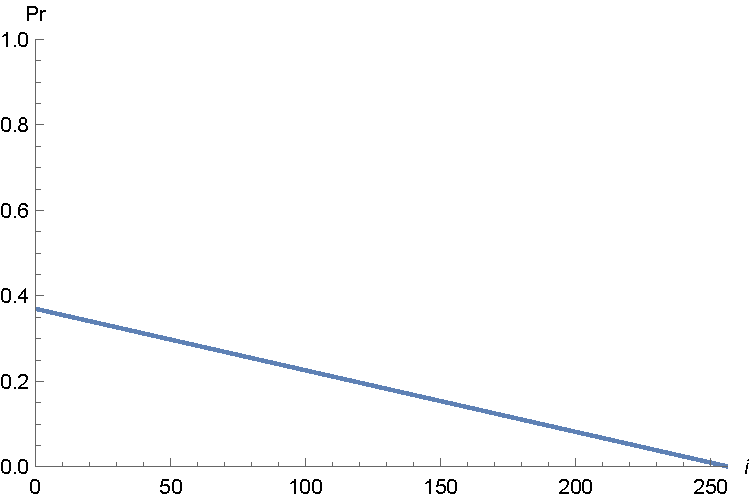
\includegraphics[width=0.7\linewidth]{img/lemma2}
		\caption{$ \Pr(S_{N}[i] = j_{i+1})  $}
		\label{fig:lemma2}
	\end{figure}


	\begin{enumerate}
		\item $ S_{r}[r] = r $ for $ r \in \FromTo{0}{i} $, i.e. the value on index $ r $ was not swapped before the $ r $-th iteration. \red{lemma 1}
		\item $ S_{i}[j_{i+1}]  = j_{i+1}$, which happens if the index $ j_{i+1} $ was not involved in previous rounds as in \red{lemma 2}
		\item $ j_{r} \neq i $ for $ r \in \FromTo{i+1}{N-1}$, i.e. $ S[i] $ is involved in any of the remaining rounds. \red{as in lemma 2}
	\end{enumerate} 

	%%%%%%%%%%% Theorem 1 S = sum of keys plus something                %%%%%%%%%%%%
	\begin{thm}{\cite{GoMa}}
		Assume that during the KSA the index j takes its values uniformly at random from $ \Z_{N} $. Then
		$ \forall i \in \Z_{Nd} $
		
		 \begin{equation}\label{theorem1}
		 \Pr(S_{N}[i] = \K{0}{i} + \dfrac{i(i+1)}{2})   \approx \bigg(\dfrac{N - i}{N}\bigg)\bigg(\dfrac{N-1}{1}\bigg)^{\frac{i(i+1)}{2}+N}+\dfrac{1}{N} 
		 \end{equation}
	\end{thm}

	\begin{proof}
		The underlying assumptions are:
		
	

	    Let $ A_{i} $ denote event that $ \forall r \in \FromTo{0}{i} S_{r}[r] = r $ as in Lemma \red{odkaz}.
	    
	    
		One way to obtain the result is by combining \red{Lemma 1 and Lemma 2} together. We have
		\[ S_{N}[i] = S_{i+1} = j_{i+1} = \sum_{r=0}^{i}(i + K[r]) \]
		with probability \red{co zbytek lemmatu 1? Proc se nepocita najednou s random association?}
		\begin{align*}
			 \Pr(A_{i})\cdot\Pr( S_{N}[i] = j_{i+1}) 
				 &= \bigg(\dfrac{N-1}{N}\bigg)^{\frac{i(i+1)}{2}}\bigg(\dfrac{N-i}{N}\bigg)\bigg(\dfrac{N-1}{N}\bigg)^{N-1} \\
				 &= \bigg(\dfrac{N-i}{N}\bigg)\cdot\bigg(\dfrac{N-1}{N}\bigg)^{\frac{i(i+1)}{2}+N-1}	
		\end{align*}
		
		Another possibility is that the event above will not happen and yet the equation holds due to random association. This 
		
		$ \left( 1 - \left(\frac{N-i}{N}\right)\cdot\left(\frac{N-1}{N}\right)^{\frac{i(i+1)}{2}+N-1} \right) \cdot \dfrac{1}{N} $
		
		
		By combining these we obtain the result as follows:
		
		$ \bigg(\dfrac{N-i}{N}\bigg)\cdot\bigg(\dfrac{N-1}{N}\bigg)^{\frac{i(i+1)}{2}+N-1} $
		+
			$ \left( 1 - \bigg(\dfrac{N-i}{N}\bigg)\cdot\bigg(\dfrac{N-1}{N}\bigg)^{\frac{i(i+1)}{2}+N-1} \right) \cdot \dfrac{1}{N} $
			
		= $ \bigg(1- \dfrac{1}{N}\bigg)	\cdot \bigg(\dfrac{N-i}{N}\bigg) \cdot \bigg(\dfrac{N-1}{N}\bigg)^{\frac{i(i+1)}{2}+N-1} + \dfrac{1}{N}$
		
		= $ \bigg(\dfrac{N-i}{N}\bigg) \cdot \bigg(\dfrac{N-1}{N}\bigg)^{\frac{i(i+1)}{2}+N} + \dfrac{1}{N}$
				
	\end{proof}
	
	

	\begin{table}[h]		
		\setlength\tabcolsep{0.035cm}
		\begin{tabular}{l@{\hspace{0.5cm}}cccccccccccccccc}
			\toprule
			i	& 0 & 1&2&3&4&5&6&7&8&9&10&11&12&13&14&15 \\
			$ 	\Pr $	& .371&.368&.364&.358&.351&.343&.334&.324&.313&.301&.288&.275&.262&.248&.234&.220\\
			\hline
			i	& 16&17&18&19&20&21&22&23&24&25&26&27&28&29&30&31 \\
			$ 	\Pr  $&	.206&.192&.179&.165&.153&.14&.129&.117&.107&.097&.087&.079&.071&.063&.056&.050 \\	
			\hline
			i   & 32&33&34&35&36&37&38&39&40&41&42&43&44&45&46&47 \\
			$ 	\Pr $ & .045&.039&.035&.031&.027&.024&.021&.019&.016&.015&.013&.011&.01&.009&.008&.008 \\
			\bottomrule
			
		\end{tabular} 
		\caption{ The probabilities of $ \ref{theorem1} $}
		\label{table:theorem1}
	\end{table}

\begin{example}
	ahpj
\end{example}


	\begin{figure}
\centering
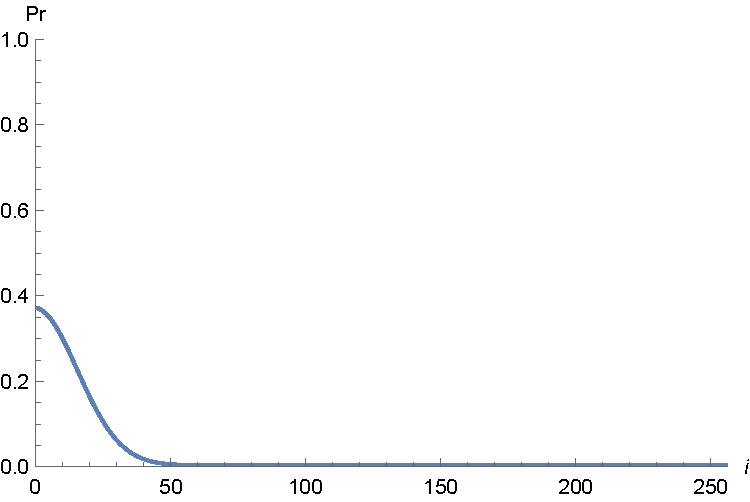
\includegraphics[width=0.7\linewidth]{img/theorem1}
\caption{}
\label{fig:theorem1}
\end{figure}

\TODO{tabulka s aktualnimi hodnotami } 



\TODO{to same pro InvS} 


\begin{thm}
	After the complete KSA, 
	\[  \Pr(S_{N}[S_{N}[i]] = \K{0}{i} + \dfrac{i(i+1)}{2}) \approx  \]
	
	clanek 4, appendix, na zacatku graf
\end{thm}

\TODO{tabulka s aktualnimi hodnotami, dukaz}


\begin{notation}
		\[  C_{i} = S_{N}[i] - \dfrac{i(i+1)}{2} \]
\end{notation}

\TODO{zobecneni na sekvence}


\TODO{inverzni sekvence}

\TODO{vyyiti tohoto na ziskani klice - rovnice} 


\section{Substracting equations}

Let $i_{1} < i_{2} $. If $ C_{i_{1}} = \K{0}{i_{1}} $ and $ C_{i_{2}} = \K{0}{i_{2}} $, then we can substract the values and get
\[ C_{i_{2}} - C_{i_{1}} = \K{0}{i_{2}} - \K{0}{i_{1}} = \K{i_{1} + 1}{i_{2}}	\].

This holds with the product of the individual probabilities of $ C_{i} $



%%%%%%%%%%% Druhy bias               %%%%%%%%%%%%
%%%%%%%%%%%%%%%%%%%%%%%%%%%%%%%%%%%%%%%%%%%%%%%%%
\section{Useful distributions for The Key Recovering Algorithm}
We can also use the fact, that with certain probability values of indices $ j_{i} $ can be found in the inner permutation or the inverse permutation and using the update rule

\[ j_{i+1} = j_{i} + S[i] + K[i\Mod{l}] \].



\begin{defn}
If $ j_{i} = S[i] $, we call this as event 1 has occured for index $ i $, and denote as $ E_{1} $.
\end{defn}

\begin{thm}
\[	P(S[i] = j_{i}) \geq (1-\dfrac{1}{N})^{i}(1-\dfrac{i-1}{N})(1-\dfrac{1}{N})^{N-i-1}+ \dfrac{1}{N} \]
\end{thm}

\begin{defn}
	If $ j_{i} = S[i] $, we call this as event 1' has occured for index $ i $, and denote as $ E'_{1} $.
\end{defn}

\begin{thm}
	\[	P(S^{-1}[i] = j_{i}) \geq (\dfrac{i}{N})(1-\dfrac{1}{N})^{N-1}+ \dfrac{1}{N}\]
\end{thm}


\begin{proof}
		$ (1-\dfrac{1}{N})^{i}(\dfrac{i}{N})(1-\dfrac{1}{N})^{N-i-1}+ \dfrac{1}{N} $
\end{proof}

\begin{thm}
	$ P(S[i] = j_{i} \vee S^{-1}[i] = j_{i}) $ used for BuildKeyTable algorithm in paper 1
\end{thm}


\TODO{ $ P(S[S[i]] = j_{i}) $ - dukazy nikde nejsou...}

\TODO{ $ P(S^{-1}[S^{-1}[i]] = j_{i}) $}

\TODO{ $ P(S[S[S[i]] = j_{i}) $}

\begin{figure}
\centering
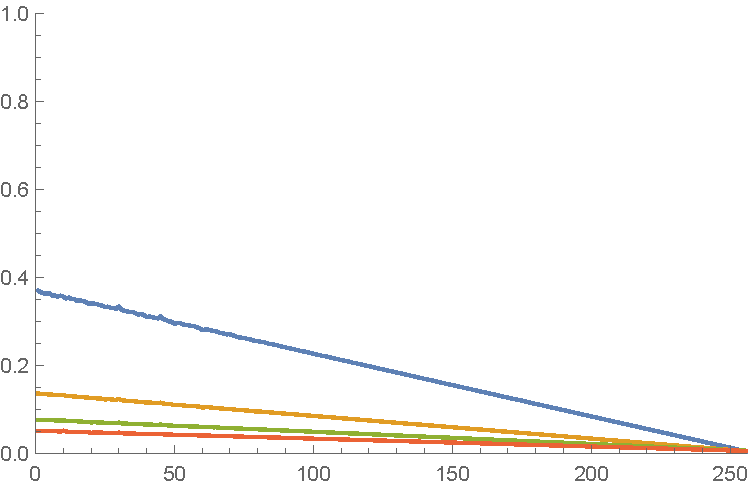
\includegraphics[width=0.7\linewidth]{img/all}
\caption[All]{hallo}
\label{fig:all}
\end{figure}


\TODO{experimentalne... rychle to konverguje}


\TODO{experimentalne vsechno dohromady je cca 0.6}


We will use both facts in the key retrieval algorithm.
